
In this chapter, we now come to the main question of this work.
We have always talked about the ``generation of supersingular curves without revealing a trapdoor'', but in fact multiple variants of this problem are conceivable.
Following \cite{base_paper}, we thus define the following three problems.
For all of these problems, we are interested in an algorithm that runs in time polynomial in $\log(p)$.
\begin{problem}[Demonstrating a hard curve]
    Given a prime $p$, compute a supersingular curve $E$ over $\F_{p^2}$ without revealing $\End(E)$.
\end{problem}
We can formalize the requirement ``without revealing $\End(E)$'' as follows.
Given $E$ and any random bits passed to the generation algorithm, it should be impossible to compute $\End(E)$.
This of course excludes random walk-based methods, since the random bits used for the random walk allows us to repeat the walk, and so find an isogeny $E_0 \to E$ from the starting curve $E_0$.
Using that isogeny, we then can compute $\End(E)$ (assuming we know $\End(E_0)$).
Furthermore, it excludes methods that yield curves with very small endomorphism ring, as those endomorphism rings are always efficiently computable.

Note that an algorithm solving the hard curve demonstration problem does not have to be randomized.
In fact, it would already be interesting to find just a single hard curve over $\F_{p^2}$ for which nobody knows the endomorphism ring.
This is different for the next problem.
\begin{problem}[Generating a random hard curve]
    Given a prime $p$, compute a random supersingular curve $E$ uniformly selected from some exponentially sized set of supersingular curves over $\F_{p^2}$, without revealing $\End(E)$.
\end{problem}
In particular, a solution to the problem can then be used to setup any cryptographic primitive with hard and secure starting curves.

Finally, the most difficult problem is to find a trapdoor-free hash function to the whole set of supersingular curves.
\begin{problem}[Hashing into hard curves]
    Given a prime $p$ and an input string $s$, deterministically find a supersingular curve $E$ without revealing $\End(E)$.
    Furthermore, if $s$ is uniform on $\{0, 1\}^n$ for a sufficiently large $n$, the resulting curve $E$ should be uniform among all supersingular curves over $\F_{p^2}$.
\end{problem}
An algorithm solving the above problem can then easily be made into a collision-free hash function by prepending it with a secure hash function.
Note that for most applications, it would already be sufficient if the above problems could be solved only for certain primes $p$. 

Next, we want to present some of the known methods to generate supersingular elliptic curves, and discuss why (or why not) they can solve one of the above problems.
After that, we introduce the idea of Katherine Stange, which is the second proposal of \cite{base_paper}.
We discuss both the theoretical and implementation issues in detail, and then prove our main result, Prop.~\ref{prop:main_result1}.
Finally, we present a modified version and prove some results on the associated distribution of supersingular curves, which includes our second main result, Prop.~\ref{prop:main_result2} and an analysis of another case.
We conclude by giving an idea that might help with performing the computations that go with our modified approach efficiently. 

\section{Naive and classical approaches}
\label{prop:naive_classical_approaches}
First, we have a look at some simple or well-known approaches to the problem, to get a feeling for the challenges.

\paragraph{Random Sampling} It is a folklore knowledge that all supersingular curves over $\bar{\F}_p$ have a j-invariant in $\F_{p^2}$, i.e. are isomorphic to a curve defined over $\F_{p^2}$.
Hence, the most naive approach is to sample random $j \in \F_{p^2}$ and check if they define supersingular curves.
It is clear that this algorithm does not reveal any information about isogenies or the endomorphism ring of the found curve, unless the information can be efficiently computed from the curve itself (in which case the cryptographic schemes are broken anyway).
However, the number of supersingular curves over $\F_{p^2}$ is only approximately $p/12$, which means that the expected number of required samples (and supersingularity checks) is about $12p$, which is exponential in $\log(p)$.

\paragraph{Random Walk} Opposed to that we have the way supersingular curves are currently generated:
As discussed in Section~\ref{sec:supersingular_isogeny_graph}, a random walk of length polynomial in $\log(p)$ in the supersingular $l$-isogeny graph is sufficient to find an (almost) uniformly distributed supersingular curve.
As long as we know one fixed curve to start with, this is quite efficient.
However, clearly this computation reveals a power-$l$ degree isogeny to the fixed starting curve, which is exactly what we want to avoid.

\paragraph{CM methods} Using the theory of complex multiplication of curves over $\C$ and their reduction modulo primes, Brökner \cite{constructing_supersingular_curves} found an algorithm that can find supersingular curves $E$ over $\F_p$, even for astronomically large primes $p$.
This method is often combined with random walks, as these naturally require a supersingular curve to start the walk from.

However, curves generated with Brökner's method have one drawback.
Namely, the algorithm has time complexity polynomial in the discriminant of the endomorphism ring of the considered curves over $\C$, and this endomorphism ring embeds into the endomorphism ring of their reduction mod $p$.
Hence, it is only efficient when generating curves with very small endomorphism rings.
This is clearly a weakness, as small endomorphism rings can be computed efficiently, for example by an exhaustive search of all low-degree isogenies.

\paragraph{Polynomial with supersingular roots} An idea that is more similar to what we will do next, is to use the following theorem \cite[Thm~V.4.1]{arithmetic_elliptic_curves}.
\begin{prop}
    Let $p$ be an odd prime and $m = (p - 1)/2$. Then the elliptic curve given by $y^2 = x(x - 1)(x - \lambda)$ over $\F_q$ is supersingular, if and only if
    \begin{equation*}
        H_p(\lambda) := \sum_{i = 0}^m {m \choose i}^2 \lambda^i = 0
    \end{equation*}
\end{prop}
In other words, we just have to find a random root of the polynomial $H_p(X)$, which then gives rise to a random supersingular curve.
The obvious problem here is again that $p$ is exponential in the input size $\log(p)$, thus the polynomial $H_p(X)$ also has exponential degree, and it is not clear if we can find a random root efficiently.

In fact, the first idea in \cite{base_paper} tries to find a random root of this polynomial, by a method similar to the Newton-Raphson iteration.
Of course, this is challenging, because it is not even clear how to evaluate $H_p(\lambda)$ efficiently for a given $\lambda$.

\section{Katherine Stange's approach}
In our research, we mainly focused on analyzing and improving the second proposal in \cite{base_paper}, which was proposed by Katherine Stange.
It is based on the following intuition.

Since the supersingular isogeny graph is an expander, it is relatively likely that there is an $n$-isogeny between two random curves $E$ and $E'$ (for a fixed $n$).
On the other hand, this is much less likely in the ordinary case.
We expect that this still applies when we take not two random curves, but a random curve $E$ and its Frobenius conjugate $E^{(p)}$, i.e. the curve with j-invariant $j(E)^p$.
Hence, the roots of
\begin{equation*}
    \Phi_n(X, X^p)
\end{equation*}
should contain a relatively large fraction of supersingular roots over $\F_{p^2}$.
This fraction can be increased by taking e.g. a gcd like
\begin{equation*}
    f_{p, n, m} := \gcd(\Phi_n(X, X^p), \Phi_m(X, X^p))
\end{equation*}
Hence, computing a random root of such a polynomial might give us a hard supersingular curve.
This idea leads to two main open questions:
\begin{question}
    \label{question:first}
    How large is the fraction of supersingular roots of $\Phi_m(X, X^p)$ resp. $f_{p, n, m}$ among all roots in $\F_{p^2}$?
\end{question}
In particular, for the method to have any hope of success, we require the fraction to be at least $1/\mathrm{poly}(\log(p))$.

The second question is more implementation-oriented. 
\begin{question}
    \label{question:second}
    How can we efficiently compute $f_{p, n, m}$, especially if $n$ resp. $m$ are exponentially large?
    Or can we efficiently find a root in some other way?
\end{question}
In the following, we try to answer both questions.
First, we present the special case that $n = l^e$ is a prime power, and describe how this might help with computing a root of $f_{p, n, m}$.
We then explain how we might be able to use the class group action to find the fraction of supersingular roots.
Finally, we present our first main result, which answers Question~\ref{question:first} for a subset of the $m$ and $n = l^e$.
Our approaches for an efficient computation also apply to this special case.
However, we are not able to answer Question~\ref{question:second}, and only provide some hints and ideas how one might handle certain difficulties.

In the case that both $n$ and $m$ are small (i.e. polynomial in $\log(p)$), \cite{base_paper} presents an approach that can find roots of $f_{p, n, m}$ even though $p$ is exponentially large, so $\Phi_n(X, X^p)$ and $\Phi_n(X, X^p)$ have exponential degree.
The idea is to take a non-square in $\F_p$ and its square root $\delta \in \F_{p^2}$.
Then $(a + b\delta)^p = a - b\delta$ and so we can equivalently look for $x, y \in \F_p$ such that
\begin{equation*}
    \Phi_n(x + \delta y, x - \delta y) = \Phi_m(x + \delta y, x - \delta y) = 0
\end{equation*}
Hence, we look for a root in $\F_p$ of the polynomial
\begin{equation*}
    \mathrm{res}_Y(\Phi_n(X + \delta Y, X - \delta Y), \Phi_m(X + \delta Y, X - \delta Y))
\end{equation*}
Of course, for each such root $x$ we still have to check that
\begin{equation*}
    \Phi_n(x + \delta Y, x - \delta Y) \quad \text{and} \quad \Phi_m(x + \delta Y, x - \delta Y)
\end{equation*}
also have roots in $\F_p$.
All of this is possible, since the polynomials in each case have degree polynomial in $n$ resp. $m$.

However, note that the elliptic curve corresponding to a root of $f_{p, n, m}$ will have an endomorphism of degree $nm$.
If we choose both $n$ and $m$ of size polynomially large in $\log(p)$, this means the endomorphism ring has polynomial discriminant, which is a weakness.
Hence, at least one of $n$ resp. $m$ has to be super-polynomial (or better exponential) in $\log(p)$.

This of course makes it very hard to even write down or compute some properties of $\Phi_n$.
In particular, the above approach does not work anymore.
We will now study a slight modification and focus on the case that $n = l^e$ is a prime power, in which we can circumvent at least parts of the problem.

\subsection{The prime power case}
First of all, we describe how the assumption $n = l^e$ might help us to work with $\Phi_n$.
Note that $\Phi_{l^e}(j(E), j(E'))$ is equivalent to there being a cyclic $l^e$-isogeny between $E$ and $E'$.
If we relax this to just any $l^e$-isogeny and note that an $l^e$-isogeny is equal to an $l$-isogeny path of length $e$, we can instead work with the condition
\begin{equation*}
    \exists x_1, ..., x_{e - 1}: \ \Phi_l(x, x_1) = \Phi_l(x_1, x_2) = ... = \Phi_l(x_{e - 1}, y) = 0
\end{equation*}
In other words, we look for a solution to the polynomial system
\begin{equation*}
    F_{p, m, l^e} := \langle \Phi_m(x, x^p), \Phi_l(x, x_1), ..., \Phi_l(x_{e - 1}, x^p) \rangle
\end{equation*}
Of course, we can again take a non-square of $\F_p$ and its root $\delta \in \F_{p^2}$ and write $x_i = y_i + \delta z_i$.
Hence, we look for a solution in $\F_p$ of the system
\begin{equation*}
    \langle \Phi_m(y + \delta z, y - \delta z), \Phi_l(y + \delta z, y_1 + \delta z_1), ..., \Phi_l(y_{e - 1} + \delta z_{e - 1}, y - \delta z) \rangle
\end{equation*}
This polynomial system is now at least efficiently computable and representable (using a standard, i.e. non-sparse, representation).

The other advantage of this approach is that every supersingular curve $E$ has an $l^e$-isogeny to $E^{(p)}$ if $e \in \Omega(\log_l(p))$.
This follows from the presented results on expander graphs.
More concretely, Theorem~\ref{prop:supersingular_graph_ramajuan} shows that the supersingular $l$-isogeny graph over $\F_{p^2}$ is an $\epsilon$-expander for
\begin{equation*}
    \epsilon = 1 - \frac {2\sqrt{d - 1}} d = 1 - 2 \frac {\sqrt{l}} {l + 1} \geq 1 - \frac 2 {\sqrt{l}}
\end{equation*}
Thus, a random walk of length at least
\begin{equation*}
    -\log_{2/\sqrt{l}}(p/12) \leq 2 \log_l(p) = \Theta(\log_l(p))
\end{equation*}
has a nonzero probability of ending in any fixed vertex, by Prop.~\ref{prop:expander_random_walk}.

This leaves us with a polynomial system of $O(\log(p))$ unknowns and equations, which at least can be explicitly written down.
Now we want to study how big the fraction of supersingular roots is.
We use the following corollary from the OSIDH class group action, see e.g. \cite[Thm~4.3]{chenu_smith}.
\begin{corollary}
    \label{prop:osidh_class_group_action}
    There are $\Theta(\sqrt{mp})$ supersingular curves $E$ over $\F_{p^2}$ with an $m$-isogeny to $E^{(p)}$.
\end{corollary}
To begin with, by our choice of $e = \Theta(\log_l(p))$, we can assume that all supersingular j-invariants are roots of $\Phi_{l^e}(X, X^p)$, and so the number of supersingular roots is $O(\sqrt{mp})$, by the above Corollary~\ref{prop:osidh_class_group_action}.
Hence, we want to find instances of $l, e$ and $m$ such that above system has only a small amount of ordinary roots, preferably $o(\sqrt{mp})$. 

\subsection{Studying the number of ordinary roots}
To estimate the number of ordinary roots, we will of course use the class group action.
Thus, we need a bound on the class number of quadratic imaginary orders.
The next theorem puts together some classical results, in particular the famous class number formula (see e.g. \cite[Corollary~VII.5.11]{neukirch}).
\begin{theorem}
    \label{prop:class_number_bounds}
    Let $\O$ be an order in a quadratic imaginary number field with discriminant $D = d(\O)$.
    Assuming GRH, we then have for the class number $h(D) := \#\Cl(\O)$ that
    \begin{equation*}
        \Theta\left(\frac {\sqrt{|D|}} {(\log\log|D|)^2}\right) \leq h(D) \leq \Theta\left(\sqrt{|D|} (\log|D|)^2\right)
    \end{equation*}
\end{theorem}
\begin{proof}
    We assume wlog that $d_K := d(\O_K) < -4$.
    Then the Dirichlet class number formula has the form
    \begin{equation*}
        h(\O_K) = \frac {\sqrt{|d_K|}} {2\pi} L(1, \chi)
    \end{equation*}
    where
    \begin{equation*}
        \chi: \Z \to \C, \quad m \mapsto \left(\frac d m\right)
    \end{equation*}
    is a real Dirichlet character and $L(s, \chi)$ is its Dirichlet L-function.
    This follows from the general class number formula, as e.g. presented in \cite[Korollar~VII.5.11]{neukirch}.

    In \cite[Thm~1]{class_number_lower_bound}, it was proven under GRH that $L(1, \chi) \geq \Theta(\sqrt{|d_K|}\log\log|d_K|)$, and the lower bound for $\O_K$ follows.
    The upper bound can easily be proven via partial summation, and does not require GRH.
    Hence, for a maximal order, we have
    \begin{equation*}
        \Theta\left(\frac {\sqrt{|D|}} {\log\log|D|}\right) \leq h(D) \leq \Theta\left(\sqrt{|D|} \log|D|\right)
    \end{equation*}

    To transfer this result to all orders, we use Corollary~\ref{prop:class_group_order}, from which it follows that
    \begin{equation*}
        h(\O) = h(\O_K) \frac {\#(\O_K / \mathfrak{f})^*} {\#(\O / \mathfrak{f})^*}
    \end{equation*}
    where $\mathfrak{f} = f\O_K \leq \O_K$ is the largest ideal contained in $\O$.
    By Corollary~\ref{prop:unit_fraction_bound}, we now see that
    \begin{equation*}
        \phi(f)h(\O_K) \leq h(\O) \leq \psi(f)h(\O_K)
    \end{equation*}
    It is a well-known fact that $\phi(f)$ is lower bounded by $\Omega(f/\log\log(f))$, and in \cite{upper_bound_dedekind_psi} it was shown that also $\psi(f)$ is upper bounded by $O(f\log\log(f)) \leq O(f\log(f))$.
    The claim now follows, since $\sqrt{|D|} = f \sqrt{|d_K|}$.
\end{proof}
Now let us come back to our estimate of the number of ordinary roots of $f_{p, m, n}$ resp. our polynomial system $F_{p, m, l^e}$.
First, we now explain why instead of (isomorphism classes of) curves it suffices to count endomorphism rings.

Whenever we have two ordinary curves $E$ and $E'$ with same endomorphism ring $\O$ in a quadratic imaginary number field $K$, then by the class group action, there is $\a \leq \O$ with $[\a].E = E'$.
Denote by
\begin{equation*}
    \Ell(\O) := \{ \text{$E$ elliptic curve} \ | \ \End(E) \cong \O \}
\end{equation*}
the set of elliptic curves with endomorphism ring $\O$.
Now the subgraph $G$ of $\Gamma_l(\F_q)$ induced by all the connected components of curves in $\Ell(\O)$ is a collection of isomorphic volcanoes.
The reason for this is the volcano structure theorem, Theorem~\ref{prop:isogeny_vulcano}, from which it follows that the structure of a volcano is determined just by the endomorphism ring of the curves on its crater.

Now consider the map
\begin{equation*}
    \Ell(\O) \to \Ell(\O), \quad E \mapsto [\a].E
\end{equation*}
It is not hard to see that this extends to a graph automorphism of $G$, again by the volcano structure.
However, it will then be not just a graph automorphism (i.e. preserves the graph structure), but also preserves Frobenius conjugates and the property of being defined over $\F_p$.
The latter follows, since being defined over $\F_p$ is a property of the endomorphism ring, namely equivalent to the ideal $(p, \pi)$ being principal.

Since our approach only uses properties of the $l$-isogeny graph and Frobenius conjugates, this means that if $E$ and $E'$ have the same endomorphism ring, it holds
\begin{equation*}
    f_{p, n, m}(j(E)) = 0 \quad \Leftrightarrow \quad f_{p, n, m}(j(E')) = 0
\end{equation*}
and similar for the system $F_{p, n, l^e}$.

Hence, we determine the set of endomorphism rings such that any (or equivalently all) corresponding curves are roots of the polynomials.
Then, the total number of curves is given by the sum over the class numbers $\sum_D h(D)$ where $D$ runs through the discriminants of said endomorphism rings. 

We mentioned before that $\Phi_m(X, X^p)$ has about $mp$ ordinary roots over $\bar{\F}_p$, but the argument implicitly assumed that the polynomial is separable.
Using endomorphism rings, it is now easy to properly lower bound the number of ordinary roots of $\Phi_m(X, X^p)$, as these correspond to the endomorphism rings with cyclic
\footnote{An element $\alpha \in \O$ is cyclic if the corresponding endomorphisms of curves $E$ with $\End(E) \cong \O$ are cyclic. This is equivalent to $n \notdivides \alpha$ for all $n \geq 2$.}
elements of norm $mp$. 
The reason is that this is equivalent to there being a solution $x \perp y$ of the Diophantine equation
\begin{equation*}
    x^2 + g y^2 = m p
\end{equation*}
where $\End(E) \cong \Z[\sqrt{g}]$, i.e. $D := d(\End(E)) = 4g$.
Note that we want a lower bound (we have an upper bound by the degree argument), and so we can ignore the possibilities in which $\End(E)$ is not of this form (i.e. $\End(E) \cong \Z[(1 + \sqrt{g})/2]$).

Furthermore, at the moment we content ourselves with a very crude estimate, but note that everything can be made rigorous.
We do that later with a very similar argument in Prop.~\ref{prop:counting_fp2_vulcano_levels}.
Neglecting $\log$-factors, we now have
\begin{align*}
    &\#\{ j \in \bar{\F}_p \ | \ \Phi_m(j, j^p) = 0 \} \geq \sum_{\substack{\text{$x^2 - gy^2 = mp$ solvable}\\\text{with $x \perp y$}}} h(4g) \\
    \geq& \sum_{0 < x < \sqrt{mp}} h(4x^2 - 4m p) \approx \sum_{0 < x < \sqrt{mp}} 2\sqrt{mp - x^2} \\
    \approx& \ 2\int_0^{\sqrt{mp}} \sqrt{mp - x^2} dx = 2mp \int_0^1 \sqrt{1 - x^2} dx \in \Omega(m p)
\end{align*}
None of the ways we consider to capture supersingularity by modular polynomials can completely exclude ordinary roots.
This is because an ordinary curve defined over $\F_p$ with endomorphisms of degree $m$ and $l$ will always be a root.
Similar situations can occur with other polynomial systems, but it is always the case that these ordinary curves have very small endomorphisms.
The next statement shows that this is not a problem, as those ordinary roots are very rare.
\begin{prop}
    \label{prop:small_endomorphism_rare}
    For $n > 0$, there are at most $O(n^{3/2}\log(n)^2)$ isomorphism classes of ordinary curves who have a non-integer endomorphism of degree $n$.
\end{prop}
\begin{proof}
    Assume that $\O$ is an imaginary quadratic order with $p \notdivides d(\O)$ that has a non-integer element $\beta \in \O \setminus \Z$ of norm $n$.
    The discriminant of the order $\Z[\beta]$ is $d(\Z[\beta]) = \mathrm{Tr}(\beta)^2 - 4\Norm(\beta) \geq -4\Norm(\beta)$.
    Hence $|d(\O)| \leq 4n$, and we find that the number of isomorphism classes of ordinary curves with a non-integer $n$-endomorphism is bounded by
    \begin{align*}
        \sum_{\substack{-4n \leq D \leq 0\\\mathclap{\text{$D$ fundamental discriminant}}}} h(D) \leq \sum_{1 \leq D \leq 4n} \sqrt{D}\log(D)^2 \in O(n^{3/2}\log(n)^2)
    \end{align*}
    This shows the claim.
\end{proof}
This is now as far as we can go in the general case.
The main problem is that once we want to determine which endomorphism rings have non-integer endomorphisms of two different degrees (e.g. $m$ and $l^e$), there is no analogue of the simple statement
\begin{equation*}
    \{ d(\O) \ | \ \text{$\O$ has cyclic endomorphism of degree $m$}\} \supseteq \{ 4(m - x^2) \ | \ 0 < x < \sqrt{m} \}
\end{equation*}
and an appropriate converse.

While the Diophantine equation $x^2 + \frac D 4 y^2 = m$ has been thoroughly studied (see e.g. \cite{cox_primes_of_form}), the best characterization for it being solvable (assuming $m = p$ is prime) involves the so-called Hilbert class polynomial
\begin{equation*}
    h_D(x) = \prod_{d(\End(E)) = D} (X - j(E))
\end{equation*}
In our case, $D$ is variable, which makes working with Hilbert class polynomials very unwieldy.
All in all, it seems like the general case is very hard to get a handle on.

\subsection{A working example}
While we are unlikely to get nice provable bounds on the number of ordinary roots in the general situation of $F_{p, m, l^e}$, there are special cases in which this is possible.
In particular, if we choose $m$ such that there is a simple relationship between $\Phi_m$ and $\Phi_{l^e}$, we can do something.
One situation in which everything works out is presented next.
In contrast to most of the other arguments we make in this section, here we argue (almost) solely with the structure of isogeny volcanoes.
\begin{prop}
    Let $l$ be a prime and further $f$ be odd and $e$ be even.
    Then the system
    \begin{equation*}
        F_{p, l^f, l^e} := \langle \Phi_{l^f}(x, x^p), \Phi_l(x, x_1), ..., \Phi_l(x_{e - 1}, x^p) \rangle
    \end{equation*}
    has $O(l^{3f}\log(l^f)^2)$ ordinary roots in $\F_{p^2}$
    \footnote{It might be not totally clear what we mean by an ordinary root of the system.
    So let us define the number of ordinary roots as the number of $j \in \bar{\F}_p$ such that $F_{p, l^f, l^e}(j, x_1, ..., x_{e - 1})$ has a solution.
    However, note that for a fixed $j$, the number of different solutions of the system is polynomial, hence it would not make a big difference if we counted all solution tuples $(x, x_1, ..., x_{e - 1})$.}.
\end{prop}
\begin{proof}
    We show that every ordinary root $j \in \F_{p^2}$ of $F_{p, l^f, l^e}$ has an endomorphism of degree at most $l^{2f}$ and the claim follows by Prop.~\ref{prop:small_endomorphism_rare}.

    For any ordinary curve $E$, denote now by $E_R$ the unique vertex in the crater of the $l$-isogeny volcano of $E$ that is connected to the lava flow tree of $E$ (in particular, $E_R = E$ if $E$ already lies on the crater).
    In other words, if $E$ is on the $i$-th lava flow tree level, then there is a sequence of ascending $l$-isogenies
    \begin{equation*}
        E = E_0 \to E_1 \to ... \to E_i = E_R
    \end{equation*}
    and $\End(E_R)$ is maximal at $l$ (meaning $l \notdivides [\O_{\End(E_R) \otimes \Q} : \End(E_R)]$).

    Note further that $(E^{(p)})_R = E_R^{(p)}$ for all ordinary curves $E$, by the functoriality of $\cdot^{(p)}$.

    Now assume a root $j$ of $F_{p, l^f, l^e}$ gives an ordinary curve $E$.
    We distinguish two cases.

    \begin{figure}
        \begin{center}
            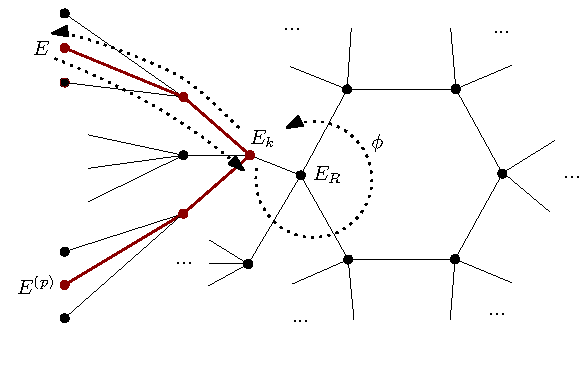
\includegraphics{./vulcano_sketch2.pdf}
        \end{center}
        \caption{\label{fig:fp_case}
            A sketch of the volcano in the case that $j(E_R) \in \F_p$ but $j(E) \notin \F_p$.
            The dotted path up to $E_k$ is then a small endomorphism of $E$, since we assume that $\phi$ is small.
            Furthermore, the path does not backtrack, as $\phi$ is cyclic and nontrivial.
        }
    \end{figure}

    If $j(E_R) \in \F_p$, i.e. the crater of the volcano is defined over $\F_p$, then clearly $E_R = (E^{(p)})_R$ (displayed in Figure~\ref{fig:fp_case}).
    Now let $k$ be minimal such that $j(E_k) \in \F_p$.
    Then every cyclic isogeny $E \to E^{(p)}$ has the form
    \begin{equation*}
        E \to E_1 \to ... \to E_k \ \overset{\phi}{\longrightarrow} \ E_k = E_k^{(p)} \to E_{k - 1}^{(p)} \to ... \to E^{(p)}
    \end{equation*}
    where $\phi$ is a power-of-$l$ endomorphism of $E_k$.

    If we apply this to the $l$-isogeny path $E \to E^{(p)}$ of length $f$, we see that $\phi$ is an $l^{f - 2i}$-endomorphism of $E_i$.
    However, since $f - 2i$ is odd by assumption, $\deg(\phi)$ is not a square and so $\phi$ is not an integer.
    This now gives a non-integer endomorphism
    \begin{equation*}
        E \to E_1 \to ... \to E_i \ \overset{\phi}{\longrightarrow} \ E_i \to E_{i - 1} \to ... \to E
    \end{equation*}
    of $E$ with degree $l^f$ and we are done.

    If $j(E_R) \notin \F_p$, then $E_R \not\cong E^{(p)}_R$.
    In particular, this means that the ideal $(p, \pi)$ in $\O := \End(E_R)$ is non-principal.
    Now we consider the subcases how $(l)$ splits in $\O$.
    
    \begin{figure}
        \begin{center}
            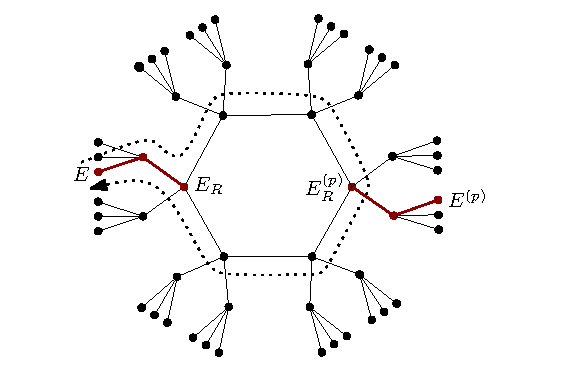
\includegraphics{./vulcano_sketch1.pdf}
        \end{center}
        \caption{\label{fig:split_case} 
            A sketch of the volcano in the case that $j(E_R) \in \F_{p^2} \setminus \F_p$ and $l$ splits in $\O_K$.
            Since $E_R$ is defined over $\F_{p^2}$, we know that $[(p, \pi)]^2.E_R = E_R$ and so $E_R^{(p)}$ is on the opposite side of the volcano.
            Now we can take the dotted path around the crater and find a small endomorphism of $E$.
        }
    \end{figure}

    If $(l) = \l_1 \l_2$ is split in $\O$ (see also Figure~\ref{fig:split_case}), note that our cyclic $l$-isogeny path $E \to E^{(p)}$ of length $f$ induces a path $E_R \to E_R^{(p)}$ of length $f - 2i$, for some $i \geq 0$.
    Since walking around the crater is given by the action of $\l_1$, we see that $[(p, \pi)] = [\l_1]^{f - 2i}$ in the ideal class group.
    Thus $\l_1^{2f - 4i}$ is principal ($E_R$ is defined over $\F_{p^2}$, so $[(p, \pi)]^2 = 1$), and its generator gives a non-integer endomorphism $\phi$ of $\End(E_R)$ of degree $l^{2f - 4i}$.
    Now
    \begin{equation*}
        E = E_0 \to E_1 \to ... \to E_i = E_R \ \overset{\phi}{\longrightarrow} E_R = E_i \to E_{i - 1} \to ... \to E
    \end{equation*}
    gives a non-integer endomorphism of $E$ with degree $l^{2f - 2i} \leq l^{2f}$, so we are done.

    If $(l)$ is inert in $\O$, the crater only has a single vertex.
    Since we have $E_R \not\cong E_R^{(p)}$ are both curves in a crater, we see that they must be in different $l$-isogeny volcanoes.
    Hence, this also holds for $E$ and $E^{(p)}$ and there cannot be an $l^f$-isogeny $E \to E^{(p)}$, contradicting our assumption.

    Finally, we are left with the case that $(l) = \l^2$ is ramified in $\O$ (see Figure~\ref{fig:ramified_case}).
    This is the only case where we will use the fact there is also an $l$-isogeny path $E \to E^{(p)}$ of length $e$.
    Since $(l)$ is ramified, we see that the crater of the volcano has exactly two vertices, which then must be $E_R$ and $E_R^{(p)}$.

    \begin{figure}
        \begin{center}
            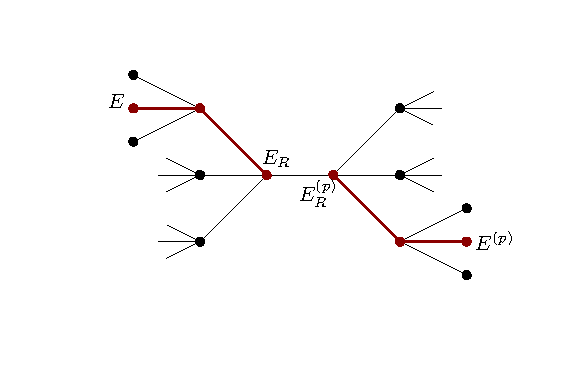
\includegraphics{./vulcano_sketch3.pdf}
        \end{center}
        \caption{\label{fig:ramified_case}
            A sketch of the volcano in the case that $j(E_R) \in \F_{p^2} \setminus \F_p$ and $l$ is ramified in $\O_K$.
            In this graph, there is no path from $E$ to $E^{(p)}$ of even length.
        }
    \end{figure}

    We did not assume that the $l$-isogeny path $E \to E^{(p)}$ of length $e$ does not backtrack.
    But we can still remove the backtracks, and get a cyclic path $E \to E^{(p)}$ of length $e - 2k$, where $k$ is the number of backtracking steps in the original path.
    Now this new path must go through the crater, and thus is of the form
    \begin{equation*}
        E = E_0 \to E_1 \to ... \to E_i = E_R \to E_R^{(p)} = E_i^{(p)} \to E_{i - 1}^{(p)} \to ... \to E_0^{(p)} = E^{(p)}
    \end{equation*}
    However, now we get a contradiction, since above path has odd length $2i + 1$, while $e - 2k$ is even by assumption.
\end{proof}
By choosing $e = \Theta(\log_l(p))$, we have $\Theta(\sqrt{l^fp})$ supersingular roots of above system.
Thus, this theorem shows that the fraction of supersingular roots is not just noticeable, i.e. $1/\mathrm{poly}(\log(p))$, but even exponentially large.
In particular, this proves our main result Prop.~\ref{prop:main_result1} and answers Question~\ref{question:first} in the considered case.
Furthermore an algorithm that is able to efficiently compute a random root of $F_{p, l^f, l^e}$ over $\F_{p^2}$ can be used to generate a random supersingular curve with very high probability.
We expect that this will not reveal a trapdoor, i.e. information about the endomorphism ring.

Note that we can choose $f$ very small, e.g. $\log_l\log(p)$ and thus $n = l^f$ is polynomial in $\log(p)$.
Therefore, we can indeed write down the system
\begin{equation*}
    F_{p, l^f, l^e} := \langle \Phi_{l^f}(x, x^p), \Phi_l(x, x_1), ..., \Phi_l(x_{e - 1}, x^p) \rangle
\end{equation*}
explicitly.
Next, we try to demonstrate this in one example.
\begin{example}
    Assume we choose $p = 51$, $l = 3$, $f = 3$ and $e = 4$.
    Then $e$ is somewhat smaller than the bound required to have $\Phi_{l^e}(j_1, j_2) = 0$ for all supersingular $j_1$, $j_2$.
    Still, we expect that most roots of $f_{p, l^f, l^e}$ are supersingular.
    We have that
    \begin{align*}
        \Phi_3 =& -x^3y^3 + 6x^3y^2 + 6x^2y^3 + x^4 + 8x^3y + 7x^2y^2 + 8xy^3 + y^4 + 9x^3 \\
        &+ 12x^2y + 12xy^2 + 9y^3 - 26x^2 + 5xy - 26y^2 - 26x - 26y
    \end{align*}
    and hence, $\Phi_{l^f}$ and $\Phi_{l^e}$ are huge, having 1240 resp. 11162 monomials.
    However, we can still compute $f_{p, l^f, l^e}$, which is a polynomial of degree $156$.
    It has the $F_{p^2}$-roots
    \begin{equation*}
        39, 52\alpha + 42, \alpha + 38, 0, 46, 44\alpha + 46, 9\alpha + 10, 50
    \end{equation*}
    Of those, $0$, $50$, $46$, $9\alpha + 10$ and $44\alpha + 46$ are supersingular, and the other three are ordinary.
    The corresponding $3$-isogeny graphs are displayed in Figure~\ref{fig:example_51}.
    Note that all ordinary solutions are in a volcano with a curve that has a non-integer $3$-endomorphism.
    \begin{figure}
        \begin{minipage}{0.5\textwidth}
            \centering
            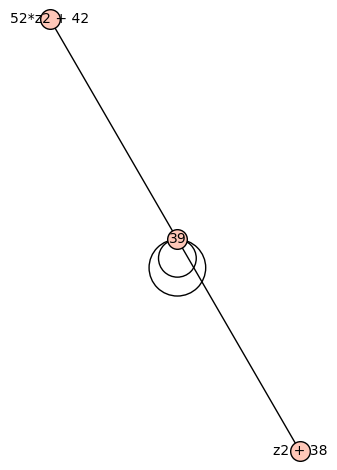
\includegraphics[width = 0.75\textwidth]{../example_51_ordinary.png}
        \end{minipage}%
        \begin{minipage}{0.5\textwidth}
            \centering
            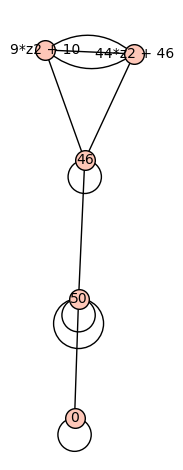
\includegraphics[width = 0.45\textwidth]{../example_51_supersingular.png}
        \end{minipage}
        \caption{\label{fig:example_51} Ordinary 3-isogeny volcano (left) and supersingular 3-isogeny graph (right) over $\F_{51^2}$, where $\mathrm{z2} = \alpha$ is a generator of $\F_{51^2}$.}
    \end{figure}
\end{example}
It is a fact that this example cannot completely show that the method works, and most roots are supersingular.
It would be much preferable if we could choose larger parameters, such that $\sqrt{p}$ and polynomial in $\log(p)$ look very different.
However, we very soon hit the limits of computers - just remember that $\Phi_{3^4}$ already has 11162 monomials.

Also the standard approach using Groebner basis does not work, as we expect its complexity to be exponential in the number of variables, i.e. exponential in $\log_l(p)$.
Already for $l = 3$ and $e = 4$, it is very slow and takes time in the range of minutes.
The original paper~\cite{base_paper} mentioned it might be possible to use a ``square-and-multiply'' approach to compute the resultant
\begin{equation*}
    \mathrm{res}_Y(\Phi_n(X + \delta Y, X - \delta Y), \Phi_{l^e}(X + \delta Y, X - \delta Y))
\end{equation*}
for some $\delta = \sqrt{a}$ with a non-square $a \in \F_p^*$.
However this means we will not represent $\Phi_{l^e}$ by the polynomial system anymore, hence we would need to get enough information about the exponential-degree modular polynomial $\Phi_{l^e}$ another way.
This seems to be a very serious obstacle.

\section{An idea based on Sutherland's supersingularity test}
As an alternative to the above approach, we propose another set of polynomial equations, whose properties might make computations easier.
In particular, our system does not consist of long dependency cycles, in the sense that we have equations $f_i(x_i, x_{i + 1})$ and $f_n(x_n, x_0)$.
Instead, our equations are of the form $f_i(x_i, x_{i + 1})$ and $f_n(x_n)$, which seems to be easier to handle.

The basic idea is to use Sutherland's supersingularity test (see Section~\ref{sec:sutherlands_supersingularity_test}).
Namely, if we take three non-backtracking walks away from an ordinary starting curve $E_0$ (such that the second vertices are distinct), then at least one of them will descend into a lava flow, and encounter a curve not defined over $\F_{p^2}$ after polynomially many steps.
On the other hand, if we do the same starting from a supersingular curve, this will not happen, as the whole supersingular isogeny graph is defined over $\F_{p^2}$.

We have already seen that $\log_l(p)$ steps are sufficient, which is also Sutherland's original choice.
However, this is not optimal, and in our case, we are also interested in how many ordinary curves we will accept if we choose $n$ smaller than the optimal bound.
In particular, our method can deal with a small number of ordinary roots (e.g. polynomially many), it should just not exponentially exceed the number of supersingular roots.
All this is considered in the next two propositions, which are again phrased in the language of endomorphism rings.
\begin{prop}
    \label{prop:frobenius_in_nonmaximal_order}
    Let $p$ be an odd prime and $m \geq 2$ an integer.
    Consider the number $n$ of endomorphism rings $\O$ of ordinary curves defined over $\F_{p^2}$ with $\pi \in \Z + m\O$, where $\pi$ is the $p^2$-Frobenius endomorphism of $\O$.
    Then
    \begin{equation*}
        \Bigl\lfloor \frac {2p} {m^2} \Bigr\rfloor \leq n \leq \Bigl\lfloor \frac {2p^2} {m^2} \Bigr\rfloor
    \end{equation*}
    Furthermore, consider the number $N$ of ordinary j-invariants $j \in \F_{p^2}$ such that $\pi \in \Z + m\End(j)$.
    Under GRH, we have then for $m^2 \leq 2p$ that
    \begin{equation*}
        \Theta\left( \frac {p^2} {m^3 \log\log(p)^2} \right) \leq N \leq \Theta\left( \frac {p^3\log(p)^2} {m^3} \right)
    \end{equation*}
    Finally, if $m^2 \geq 4p^2$, we have $n = N = 0$.
\end{prop}
\begin{proof}
    First, we show the lower bounds.
    Note that there are $\lfloor 2p/m^2 \rfloor$ different integers $a$ with $0 < am^2 < 2p$ (clearly $m^2 \notdivides 2p$).
    For each of them, consider $g = am^2(am^2 - 2p)$.
    We have
    \begin{equation*}
        (p - am^2)^2 - g \cdot 1^2 = p^2 - 2pam^2 + a^2m^4 - a^2m^4 + 2pam^2 = p^2
    \end{equation*}
    Thus the imaginary quadratic order $\O := \Z[\sqrt{g}]$ with discriminant $D := 4g$ contains a non-integer element of norm $p^2$, which must be the Frobenius $\pi$ (or its conjugate).
    In particular, the imaginary quadratic order $\O_0$ with discriminant $d := D/m^2$ satisfies $\O = \Z + m\O_0$ as $[\O_0 : \O]^2 = d(\O)/d(\O_0) = m^2$
    Therefore we see that $\pi \in \Z + m\O_0$.
    Note that each $a$ gives rise to a distinct $\O_0$, since $d(\O_0) = 4a(am^2 - 2p)$, and the first lower bound follows.

    To get a lower bound for the number of curves, note that for each $\O_0$, by the class group action, there are exactly $\#\Cl(\O_0)$ curves with that endomorphism ring.
    Under GRH, Theorem~\ref{prop:class_number_bounds} gives
    \begin{equation*}
        h(D) \geq \frac {\sqrt{|D|}} {(\log\log|D|)^2} \Theta(1)
    \end{equation*}
    Hence, the total number of curves is lower bounded by
    \begin{align*}
        &\Theta(1) \sum_{1 \leq a \leq \lfloor 2p/m^2 \rfloor} h(4a(am^2 - 2p)) \geq \Theta(1) \sum_{1 \leq a \leq \lfloor 2p/m^2 \rceil} \frac {\sqrt{4a|am^2 - 2p|}} {(\log\log|4a(am^2 - 2p)|)^2} \\
        =& \Theta(1) m \sum_{1 \leq a \leq \lfloor 2p/m^2 \rfloor} \frac {\sqrt{a} \sqrt{2p/m^2 - a}} {(\log(\log(4) + \log(am^2) + \log(2p - am^2)))^2} \\
        \geq& \Theta(1) \frac {m} {(\log(\log(4) + 2\log(p)))^2} \sum_{1 \leq a \leq \lfloor 2p/m^2 \rfloor} \sqrt{a} \sqrt{2p/m^2 - a} \\
        =& \Theta(1) \frac {m} {\log\log(p)^2} \int_0^{2p/m^2} \sqrt{a} \sqrt{2p/m^2 - a} \ da \\
        =& \Theta(1) \frac {p^2} {m^3 \log\log(p)^2} \int_0^1 \sqrt{x(1 - x)} dx = \Theta\left( \frac {p^2} {m^3 \log\log(p)^2} \right)
    \end{align*}
    We assume that $p \geq m^2$ when estimating the sum by the integral.

    Now to the upper bounds.
    Consider an imaginary quadratic order $\O$ with $\pi \in \O$.
    Then clearly $d(\O) \divides d(\Z[\pi]) = t^2 - 4p^2$, where $t$ is the trace of $\pi$.
    Thus we see that $|d(\O)| \leq 4p^2$.
    If now $\O = \Z + m\O_0$ for some order $\O_0$, we know that
    \begin{equation*}
        d(\O) = [\O : \O_0]^2 d(\O_0) = m^2 d(\O_0)
    \end{equation*}
    and so $-4p^2/m^2 \leq d(\O_0) < 0$.
    Furthermore, only half of the $d \geq -4p^2/m^2$ are congruent to $0, 1$ modulo 4, i.e. are fundamental discriminants.
    Therefore, there are at most $\lfloor 2p^2/m^2 \rfloor$ different endomorphism rings $\O_0$ with $\pi \in \Z + m\O_0$.

    For an upper bound on the number of curves, just note that
    \begin{equation*}
        \#\{ j \in \F_{p^2} \ | \ \pi \in \Z + m\End(j) \} \leq \sum_{-4p^2/m^2 \leq D < 0} h(D)
    \end{equation*}
    Using the bound on the class number from Prop.~\ref{prop:class_number_bounds}, we can bound this by
    \begin{align*}
        &\sum_{D = 1}^{\lfloor 4p^2/m^2 \rfloor} \sqrt{D} \log(D)^2 \leq \Theta(\log(p)^2) \int_1^{\lfloor 4p^2/m^2 \rfloor + 1} \sqrt{x} dx \\
        =& \Theta(\log(p)^2) \int_0^{4p^2/m^2} \sqrt{x} dx = \Theta(\log(p)^2) \frac {4p^2} m \int_0^1 \sqrt{x} dx \\
        =& \Theta\left( \frac {p^3\log(p)^2} {m^3} \right)
    \end{align*}
    This estimate is valid, since $\sqrt{x}$ is increasing and $\sqrt{\lfloor 4p^2/m^2 \rfloor + 1} / \sqrt{4p^2/m^2} \in O(1)$.
    This shows the claim.
\end{proof}
Note that the bound for the number of curves is not very tight.
In particular, there is a factor of more that $p$ between upper and lower bound.
In the case that $m = l^e$ is a prime power (this is the case of the levels in an $l$-isogeny volcano), we get a much clearer picture.
\begin{prop}
    \label{prop:counting_fp2_vulcano_levels}
    Let $p$ be an odd prime and $m = l^e$ a prime power with $l \neq 2, p$.
    Then we have for the numbers $n$ resp. $N$ from the previous proposition~\ref{prop:frobenius_in_nonmaximal_order} the following improved upper bounds
    \begin{equation*}
        n \leq \Bigl\lfloor \frac {16p^2} {m^3} \Bigr\rfloor
    \end{equation*}
    and
    \begin{equation*}
        N \leq \Theta\left( \frac {p^2\log(p)^3} {m^3} \right)
    \end{equation*}
    Furthermore, if $m^2 > 4p$, we have that $n = N = 0$.
\end{prop}
\begin{proof}
    Consider an endomorphism ring $\O_0$ such that $\O := \Z + m\O_0$ contains the $p^2$-Frobenius $\pi$.
    Then
    \begin{equation*}
        \Z[\pi] \subseteq \O \subseteq \O_0
    \end{equation*}
    and so $D := d(\Z[\pi]) = a^2m^2d(\O_0)$ for the integer $a = [\O_K : \Z[\pi]] / m$.
    Furthermore, if $t$ is the trace of $\pi$, we find $D = t^2 - 4p^2 = (t - 2p)(t + 2p)$.
    Hence
    \begin{equation*}
        a^2m^2d(\O_0) = (t - 2p)(t + 2p)
    \end{equation*}
    Since $m$ is odd, we see that $m$ must be coprime to either $t - 2p$ or $t + 2p$ (it does not divide $4p$).
    Note that here, we use the assumption that $m$ is a prime power.

    If $m^2 \divides t + 2p$, then $t \in \{ m^2 - 2p, 2m^2 - 2p, ..., km^2 - 2p \}$ where $k = \lfloor 4p/m^2 \rfloor$.

    If $m^2 \divides t - 2p$, then $t \in \{ 2p - km^2, 2p - (k - 1)m^2, ..., 2p - m^2 \}$.
    \\
    In particular, there are at most $2k$ different choices for $t$.
    Additionally, it clearly implies that if $m^2 > 4p$, we have $k = 0$ and so $n = N = 0$.

    Otherwise, for a given $t$, there are now at most
    \begin{equation*}
        \sqrt{\frac {|t^2 - 4p^2|} {m^2}} \leq \sqrt{\frac {4p^2} {m^2}} = \frac {2p} m
    \end{equation*}
    choices for $a$, which then uniquely determines $d(\O_0)$.
    The total number of possibilities for $d(\O_0)$ is thus
    \begin{equation*}
        2k \frac {2p} {m} \leq \frac {16p^2} {m^3}
    \end{equation*}
    To bound the number of curves, we again use the class group action and the following bound on the class number of a quadratic imaginary number field.
    Namely, if the discriminant is $D$, have
    \begin{equation*}
        h(D) \leq \sqrt{|D|}(\log|D|)^2 O(1)
    \end{equation*}
    This now gives us the following upper bound on the number of curves
    \begin{align*}
        &\sum_{1 \leq i \leq k} \quad \sum_{a^2 \divides ((im^2 - 2p)^2 - 4p^2)/m^2} h\Biggl( \frac {(im^2 - 2p)^2 - 4p^2} {a^2m^2} \Biggr) \\
        &+ \sum_{1 \leq i \leq k} \quad \sum_{a^2 \divides ((2p - im^2)^2 - 4p^2)/m^2} h\Biggl( \frac {(2p - im^2)^2 - 4p^2} {a^2m^2} \Biggr) \\
        =& 2\sum_{1 \leq i \leq k} \quad \sum_{a^2 \divides ((im^2 - 2p)^2 - 4p^2)/m^2} h\Biggl( \frac {(im^2 - 2p)^2 - 4p^2} {a^2m^2} \Biggr) \\
        \leq& O(\log(4p^2/m^2)^2) \sum_{1 \leq i \leq k} \sqrt{\frac {4p^2 - (im^2 - 2p)^2} {m^2}} \sum_{a^2 \divides ((im^2 - 2p)^2 - 4p^2)/m^2} \frac 1 a
    \end{align*}
    Note that
    \begin{align*}
        \sum_{a^2 \divides x} \frac 1 a \leq \sum_{a \leq \sqrt{x}} \frac 1 a = O(\log(x))
    \end{align*}
    Thus we can upper bound the previous sum by
    \begin{align*}
        &O(\log(4p^2/m^2)^2) \sum_{1 \leq i \leq k} \sqrt{ \frac {4p^2 - (im^2 - 2p)^2} {m^2}} \quad \log\left( \frac {4p^2 - (im^2 - 2p)^2} {m^2} \right) \\
        =& \frac {O(\log(p/m)^3)} {m} \sum_{1 \leq i \leq k} \sqrt{4p^2 - (im^2 - 2p)^2} \\
        =& \frac {O(\log(p/m)^3)} {m}  \int_0^k \sqrt{4p^2 - (xm^2 - 2p)^2} dx \\
        =& \frac {O(\log(p/m)^3)} {m} \frac 1 {m^2} \int_0^{2p} \sqrt{4p^2 - (x - 2p)^2} dx \\
        =& \frac {O(\log(p/m)^3)} {m} \frac 1 {m^2} \int_{-2p}^0 \sqrt{4p^2 - x^2} dx \\
        =& \frac {O(\log(p/m)^3)} {m} \frac {4p^2} {m^2} \int_{-1}^0 \sqrt{1 - x^2} = O\left( \frac {p^2\log(p/m)^3} {m^3} \right)
    \end{align*}
    This shows the claim.
\end{proof}
This bound is quite tight, and we see that $N \approx p^2/m^3$ up to log-factors.
The distribution of the curves is also displayed in Figure~\ref{fig:number_of_fixed_level_curves}.
\begin{figure}
    \begin{center}
        \begin{tikzpicture}
            \begin{axis}[
                width = 0.8\textwidth, 
                height = 0.4\textheight, 
                axis lines = middle,
                xlabel = $p$,
                ylabel = $N$
            ]
                \pgfplotstableread{data.txt}\mydata;
                \addplot[ 
                    color = black, 
                    only marks, 
                    mark = *, 
                    mark size = 0.5pt, 
                ]
                table[
                    x expr=\thisrowno{0}, 
                    y expr=\thisrowno{1}
                ] {\mydata};
                \addplot [red, domain=1000:2650] {0.5*x^2/27^3};
            \end{axis}
        \end{tikzpicture}
    \end{center}
    \caption{
        \label{fig:number_of_fixed_level_curves} A plot of the number $N$ for $m = 3^3$ and increasing $p$.
        For reference, we also displayed the function $\frac 1 2 p^2/m^3$ in red.
        Note that $N$ is the number of curves $E$ with $\pi \in \Z + m\End(E)$, i.e. there are 3 levels defined over $\F_{p^2}$ beneath $E$ in the 3-isogeny volcano.
    }
\end{figure}
In particular, it follows that we can choose $m = l^r$ with $r = \lceil \frac 1 2 \log_l(p) \rceil$ and can be sure never to accept an ordinary curve as supersingular.
Furthermore, if we are ok with accepting $O(p)$ ordinary curves as supersingular, we can choose $r = \lceil \frac 1 3 \log_l(p) \rceil$.

\subsection{Generating curves}
According to the above discussion, the obvious polynomial system we want to find a root of is
\begin{equation*}
    \langle \Phi_m(x, y_1), \Phi_m(x, y_2), \Phi_m(x, y_3), \ y_1^{p^2 - 1} - 1, \ y_2^{p^2 - 1} - 1, \ y_3^{p^2 - 1} - 1 \rangle
\end{equation*}
Since $m$ will be exponentially large, and we have no good description of $\Phi_m$, we can again consider the paths explicitly.
More concretely, assume that $m = l^n$.
We use the polynomial system
\begin{align*}
    \langle &\Phi_l(x, u_0), \Phi_l(x, v_0), \Phi_l(x, w_0), \\
    &\Phi_l(u_0, u_1), \Phi_l(v_0, v_1), \Phi_l(w_0, w_1), \\
    &... \\
    &\Phi_l(u_{n - 1}, u_n), \Phi_l(v_{n - 1}, v_n), \Phi_l(w_{n - 1}, w_n), \\
    &u_n^{p^2 - 1} - 1, v_n^{p^2 - 1} - 1, w_n^{p^2 - 1} - 1 \rangle
\end{align*}
We can explicitly write down that system.

However, a solution to this system might ``collapse'' nodes, e.g. have $u_i = u_{i + 2}$.
Then the corresponding $l$-isogeny path backtracks, and it is not guaranteed that one path reaches the $n$-th lava flow level.
Hence, we can still get many ordinary curves.

Then condition $u_i \neq u_{i + 2}$ is not algebraically closed, so we cannot write it as a polynomial directly.
But we can use the structure of the volcanoes (in particular, they have at most one cycle), and the fact that $\Phi_m$ characterizes the existence of a \emph{cyclic} isogeny.
Hence, consider the polynomial system
\begin{align*}
    \langle &\Phi_l(x, u_0), \Phi_l(x, v_0), \Phi_l(x, w_0), \\
    &\Phi_l(u_0, u_1), \Phi_l(v_0, v_1), \Phi_l(w_0, w_1), \\
    &... \\
    &\Phi_l(u_{n - 1}, u_n), \Phi_l(v_{n - 1}, v_n), \Phi_l(w_{n - 1}, w_n), \\
    &u_n^{p^2 - 1} - 1, v_n^{p^2 - 1} - 1, w_n^{p^2 - 1} - 1, \\
    &\Phi_{l^2}(u_0, v_0), \Phi_{l^2}(u_0, w_0), \Phi_{l^2}(v_0, w_0), \\
    &\Phi_{l^2}(u_0, u_2), \Phi_{l^2}(v_0, v_2), \Phi_{l^2}(w_0, w_2), \\
    &... \rangle
\end{align*}
The additional constraints $\Phi_{l^2}(u_i, u_{i + 2})$ ensure that $u_i \neq u_{i + 2}$, unless the curve of j-invariant $u_i$ has a cyclic endomorphism of size $l^2$.
However, this means that its endomorphism ring has polynomially large discriminant, and again there are only polynomially many such curves by Prop.~\ref{prop:small_endomorphism_rare}.
Hence, a root of above system is supersingular with probability $1 - 1/\mathrm{poly}(\log(p))$. 

Still, it seems pretty impossible to efficiently compute a random root of above system.
We now present a way that looks like there is some hope to do the computations, even though there are still some serious obstacles.
\begin{prop}
    Let $\O$ be an order in a quadratic imaginary number field with $p^2$-power Frobenius $\pi$.
    Let $l_1, ..., l_r$ be distinct primes.
    Then
    \begin{equation*}
        \pi \in \Z + l_1 ... l_r \O \quad \Leftrightarrow \quad \forall i: \pi \in \Z + l_i \O
    \end{equation*}
\end{prop}
\begin{proof}
    The direction $\Rightarrow$ is clear, as $\Z + l_1 ... l_r \O \subseteq \Z + l_i\O$.
    For the other direction, choose an integral generator $\alpha$ of $\O$, i.e. $\O = \Z \oplus \alpha\Z$.
    Then $\Z + l_i\O = \Z \oplus l_i\alpha\Z$.
    Furthermore, as an element of $\O$, the Frobenius $\pi$ has a unique representation $\pi = a + b\alpha$ with integers $a$ and $b$.
    Now the assumption
    \begin{equation*}
        \pi \in \Z + l_i\O = \Z + l_i\alpha\Z
    \end{equation*}
    implies $l_i \divides b$, and so $l_1 ... l_r \divides b$.
    Thus
    \begin{equation*}
        \pi \in \Z + l_1 ... l_r \O = \Z + l_1 ... l_r \alpha \Z \qedhere
    \end{equation*}
\end{proof}
Hence, we can instead consider the sum of systems
\begin{align*}
    \sum_i \quad \langle &\Phi_{l_i}(x, u_i), \Phi_{l_i}(x, v_i), \Phi_{l_i}(x, w_i), \\
    &\Phi_{2l_i}(u_i, v_i), \Phi_{2l_i}(u_i, w_i), \Phi_{2l_i}(v_i, w_i), \\
    &u_i^{p^2 - 1} - 1, v_i^{p^2 - 1} - 1, w_i^{p^2 - 1} - 1 \rangle 
\end{align*}
for distinct primes $l_i$ with $\prod_i l_i \geq 2p$.
Note that from these results, our second main result Prop.~\ref{prop:main_result2} follows.

\subsection{A more explicit representation}
In the hope of making computations easier, we can try to transform our system further.
For this, we first need the following lemma.
\begin{lemma}
    Assume that $k$ is an algebraically closed field.
    Let $I \leq k[x, Y, B]$ be an ideal, where $Y$ and $B$ are vectors of unknowns.
    Then elimination and evaluation commute, i.e.
    \begin{equation*}
        \mathrm{ev}_{x, b}(I \cap k[x, B]) = \mathrm{ev}_{x, Y, b}(I) \cap k[x]
    \end{equation*}
    where $b \in k[x]^n$ is a vector and $\mathrm{ev}_{x, b}$ resp. $\mathrm{ev}_{x, Y, b}$ are evaluation homomorphisms.
\end{lemma}
\begin{proof}
    Taking the point of view of varieties over the algebraically closed field $k$, we see that elimination corresponds to projection (the main theorem of elimination theory), and evaluation corresponds to the intersection with a lower-dimensional subvariety.
    Clearly, both of them commute in the above sense.
\end{proof}
We can also explicitly compute the polynomial division of $y^{p^2 - 1} - 1$ modulo $\Phi_l(x, y)$.
Note that $y^{p^2 - 1} - 1$ is the only polynomial of exponential degree, and getting rid of it would be very nice.
\begin{lemma}
    \label{prop:symbolic_elimination}
    We have
    \begin{equation*}
        y^{p^2 - 1} - 1 \equiv \left(\begin{matrix*}
            y^l \\
            \vdots \\
            1
        \end{matrix*}\right)^T b - 1 \mod \Phi_l(x, y)
    \end{equation*}
    where
    \begin{equation*}
        b = A^{p^2 - l - 1} e_1 \quad \text{for the first unit vector $e_1 = \left(\begin{matrix*}
            1 \\
            0 \\
            \vdots \\
            0
        \end{matrix*}\right)$}
    \end{equation*}
    for the explicitly computable $(l + 1) \times (l + 1)$ matrix $A \in k[x]^{(l + 1) \times (l + 1)}$ given by
    \begin{equation*}
        A = \left( \begin{matrix*}
            -a_l & 1 & 0 & \dots & 0 \\
            -a_{l - 1} & 0 & 1 & \dots & 0 \\
            \vdots & \vdots & \vdots & \ddots & \vdots \\
            -a_1 & 0 & 0 & \dots & 1 \\
            -a_0 & 0 & 0 & \dots & 0
        \end{matrix*} \right) \in k[x]^{(l + 1) \times (l + 1)}
    \end{equation*}
    where
    \begin{equation*}
        \Phi_l(x, y) = \sum_{i = 0}^{l + 1} a_i(x) y^i \in k[x][y]
    \end{equation*}
    as univariate polynomial over $k[x]$.
\end{lemma}
\begin{proof}
    We just perform univariate polynomial division of $y^{p^2 - 1} - 1$ by $\Phi_l(x, y)$ in $k[x][y]$.

    Define a sequence of polynomials in $k[x, y]$ by
    \begin{equation*}
        f_0 := y^{p^2 - 1} \quad \text{and} \quad f_{i + 1} = f_i - \mathrm{lc}(f_i) \Phi_l(x, y) y^{p^2 - l - 2 - i}
    \end{equation*}
    Here, $\mathrm{lc}(f_i)$ refers to the appropriate value when considering $f_i$ as a univariate polynomial over $k[x]$, in particular $\mathrm{lc}(f_i) \in k[x]$.
    This clearly implies that $f_i \equiv f_j \mod \Phi_l(x, y)$.
    We show that
    \begin{equation*}
        f_i = \left( \begin{matrix*}
            y^{p^2 - 1 - i} \\ \vdots \\ y^{p^2 - l - 1 - i}
        \end{matrix*} \right)^T A^i e_1
    \end{equation*}

    To see that this is true, note that $f_i$ contains only the monomials $y^{p^2 - 1 - i}, ..., y^{p^2 - l - 1 - i}$ (technically, by induction hypothesis).
    Hence, we can write
    \begin{equation*}
        f_i = y^{p^2 - l - 1 - i} \sum_{j = 0}^l c_j y^j
    \end{equation*}
    Since $a_{l + 1} = 1$, it follows that
    \begin{align*}
        f_{i + 1} =& y^{p^2 - l - 1 - i} \Bigl( \sum_{j = 0}^l (c_j - c_l a_{j + 1}) y^j \Bigr) - y^{p^2 - l - 2 - i} c_l a_0 \\
        =& y^{p^2 - l - 1 - (i + 1)} \sum_{j = 0}^l (c_{j - 1} - c_l a_j) y^j
    \end{align*}
    where we define $c_{-1} = 0$.
    Now we have
    \begin{equation*}
        \left( \begin{matrix*}
            c_{l - 1} - c_l a_l \\
            \vdots \\
            c_0 - c_l a_1 \\
           - c_l a_0
        \end{matrix*} \right) = A \left( \begin{matrix*}
            c_l \\
            \vdots \\
            c_1 \\
            c_0
        \end{matrix*} \right)
    \end{equation*}
    and the claim follows.
\end{proof}
The idea is now to introduce $l + 1$ indeterminates $B$, and compute the elimination ideal
\begin{equation}
\label{eq:elimination_ideal}
\begin{split}
    \langle &\Phi_{l_i}(x, u_i), \Phi_{l_i}(x, v_i), \Phi_{l_i}(x, w_i), \\
    &\Phi_{2l_i}(u_i, v_i), \Phi_{2l_i}(u_i, w_i), \Phi_{2l_i}(v_i, w_i), \\
    &\left(\begin{matrix*}
        u_i^l \\
        \vdots \\
        1
    \end{matrix*}\right)^T B - 1, \left(\begin{matrix*}
        v_i^l \\
        \vdots \\
        1
    \end{matrix*}\right)^T B - 1, \left(\begin{matrix*}
        w_i^l \\
        \vdots \\
        1
    \end{matrix*}\right)^T B - 1 \rangle \cap k[x, B]
\end{split}
\end{equation}
This might now be done, since all polynomials we consider now are of polynomial degree.
Next, we can find polynomials $f_{i1}, ..., f_{in_i} \in k[x, B]$ that generate this ideal.
Hence, we only have to find a random joint root of the univariate polynomials
\begin{equation*}
    f_{i j}(x, b_i) \quad \text{where} \quad b_i = A_i^{p^2 - l - 1} e_1
\end{equation*}
for the matrices $A_i$ given by Lemma~\ref{prop:symbolic_elimination}.
While we cannot explicitly write down those polynomials, we can evaluate them, evaluate their derivates and perform a series of other computations.
Hence, there might be some way to find a random root of those (note that they have all $\Theta(p)$ supersingular j-invariants and polylogarithmically many ordinary j-invariants as roots).

Nevertheless, we should also mention that the computation of the elimination ideal from equation~(\ref{eq:elimination_ideal}) is not trivial either.
The product of the considered primes $l_i$ must be at least $2p$, and so the largest ones are $\Theta(\log(p)/\log\log(p))$.
In particular, we have to perform elimination in a polynomial ring with polynomially many unknowns.
Hence, a standard Groebner basis will have exponential runtime.
However, we only have to eliminate a constant number of variables, namely $u_i$, $v_i$ and $w_i$, so there might be a way to compute a ``partial'' Groebner basis that still yields generators of the elimination ideal.
We have not studied this in depth, as finding a joint root of the $f_{ij}(x, b_i)$ seems to be a more fundamental problem.
